\documentclass{article}
\usepackage{graphicx}
\usepackage{amsmath}
\usepackage{float}
\usepackage{siunitx}
\usepackage{caption}
\usepackage{subcaption}
\usepackage{hyperref}

\title{Waveform Synthesis Using a Multistage Op-Amp Function Generator}
\author{Lily Nguyen}
\date{December 6, 2025}

\begin{document}

\maketitle

% -----------------------
% Introduction and Theory
% -----------------------

\section{Introduction and Theory}

% Your lab report, even if it consists if multiple parts, should be centered around a central
% topic. In the introduction, you should introduce this topic and place it in context. When
% giving context, think of answering questions such as ”What is the purpose of this project?”,
% “Why are the techniques or tools used important?” and more. Make sure to include a circuit
% diagram and an analysis of how the circuit works. Finally, this section should include the
% concepts and equations relevant to your stated goals and the results you plan on presenting.

This project aims to design and build function generator capable of producing
square, triangle, and sine waves using operational amplifiers and discrete
components. Rather than relying on commercial waveform ICs, we implemented each
function block separately to produce these waveforms and explore principles
of signal synthesis.\\

\noindent Our circuit consists of three main stages: a square wave oscillator, a
triangle wave integrator, and a sine wave shaper, as shows in Figure~\ref{fig:block}.

\begin{figure}[H]
    \centering
    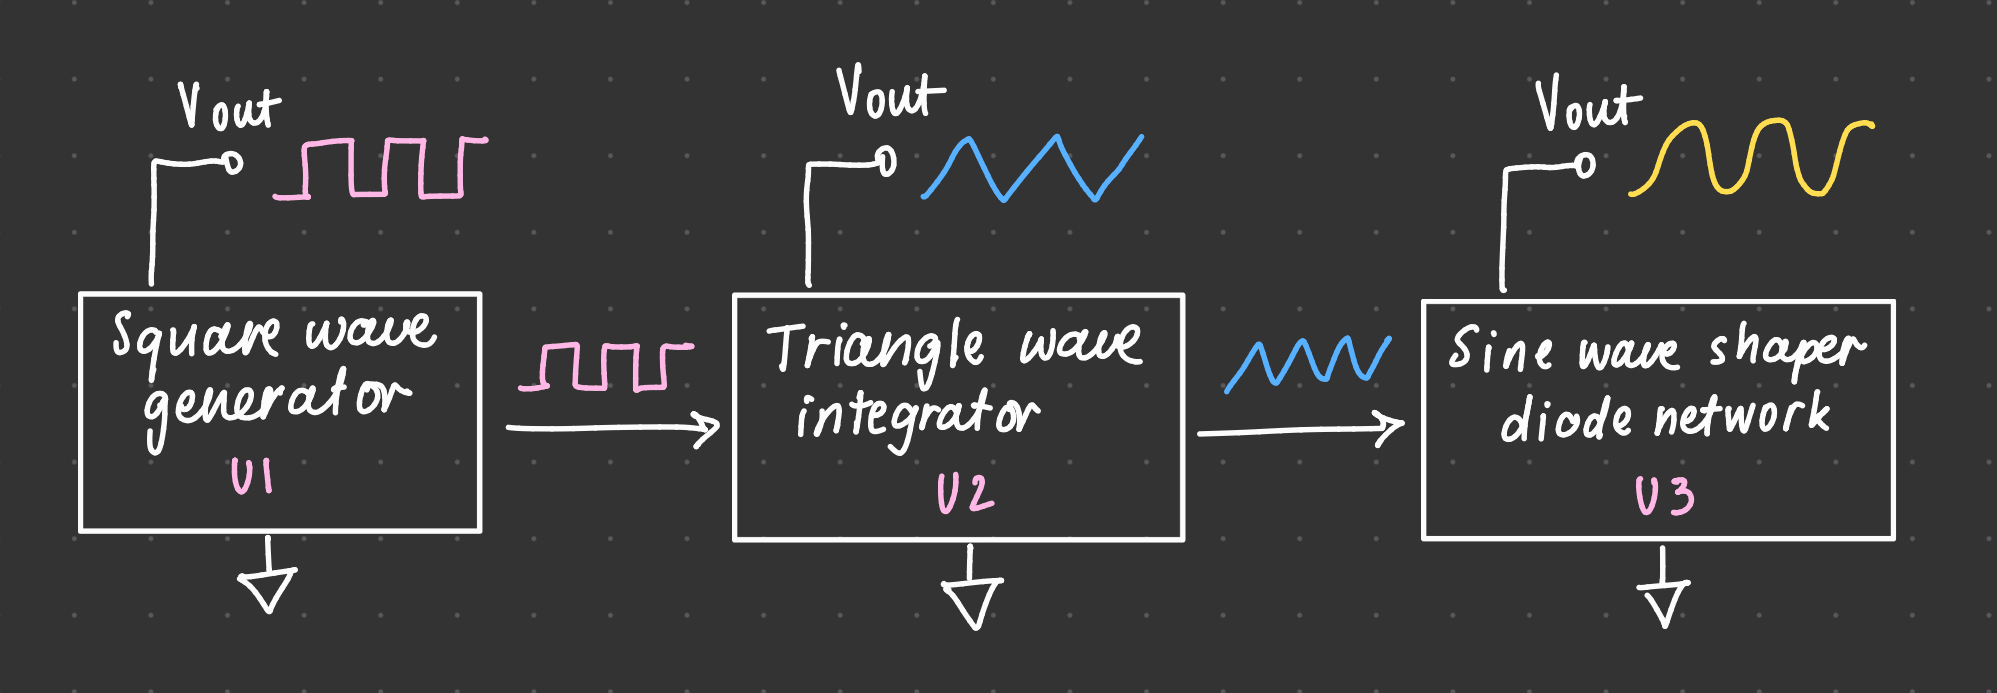
\includegraphics[width=.8\textwidth]{block.jpg}
    \caption{Block diagram of the function generator circuit. The signal flows
    the comparator-based square wave oscillator to an op-amp integrator that
    outputs a triangle wave, and finally to a nonlinear shaping circuit that
    produces a sine wave.}
    \label{fig:block}
\end{figure}

\noindent The first stage uses a comparator configuration (U1) with positive
feedback via a resistor-divider network. The op-amp toggles between the
positive and negative supply rails whenver the inverting input crosses the
threshold voltage:
\begin{equation}
    V_\text{threshold}=\pm\left(\frac{R_3}{R_1+R_3} \right)V_\text{out},
\end{equation}
\noindent where $R_1$ and $R_3$ form the voltage divider \cite{eeeguide}. The resistor $R_2$
and the capacitor in the following integrator stage define the RC
time constant that controls the output frequency. This configuration functions
similarly to a Schmitt trigger, which produces a square wave by switching
states as the capacitor charges and discarges \cite{schertz}. The charging path through $R_2$
and the feedback from the integrator ensure the timing interval stays consistent
and results in a stable waveform with well-defined frequency and symmetry.\\

\noindent The square wave generated by the comparator stage feeds into an
inverting integrator composed of an op-amp (U2), resistor $R_2$, and feedback
capacitor $C_1$. This circuit operates as an integrator by converting the
constant high and low levels of the square wave into a linearly increasing or
decreasing voltage \cite{schertz}. The resulting output is a triangle wave where $V_\text{out}$
evolves according to the relation:
\begin{equation}
    V_\text{out}(t)=-\frac{1}{RC}\int V_\text{in}(t)dt
\end{equation}
\noindent Increasing the square wave amplitude increases the rate of change,
whereas increasing the RC constant slows it down. Assuming symmetrical 
saturation and ideal integration, the frequency of oscillations is 
$f=\frac{1}{T}=\frac{R_1}{4R_2R_3C_1}$ \cite{eeeguide}.\\

\noindent To convert the triangle wave into a sine-like waveform, we use a
nonlinear shaping circuit composed of diodes and resistor. The diodes begin
conducting at specific voltage thresholds (around $0.6$-$0.7$ V), which alters
the waveform slope in a piecewise linear manner. As the triangle wave
amplitude increases, more diodes enter conduction to successively compress
the waveform peaks and round them to a better approximate sine wave. The shaped
signal is then passed through a summing amplifier, which allows for additional
gain control and centering of the output waveform around $0$ V \cite{elliott}.\\

\noindent Figure~\ref{fig:schematic} shows the full circuit schematic for our
function generator.

\begin{figure}[H]
    \centering
    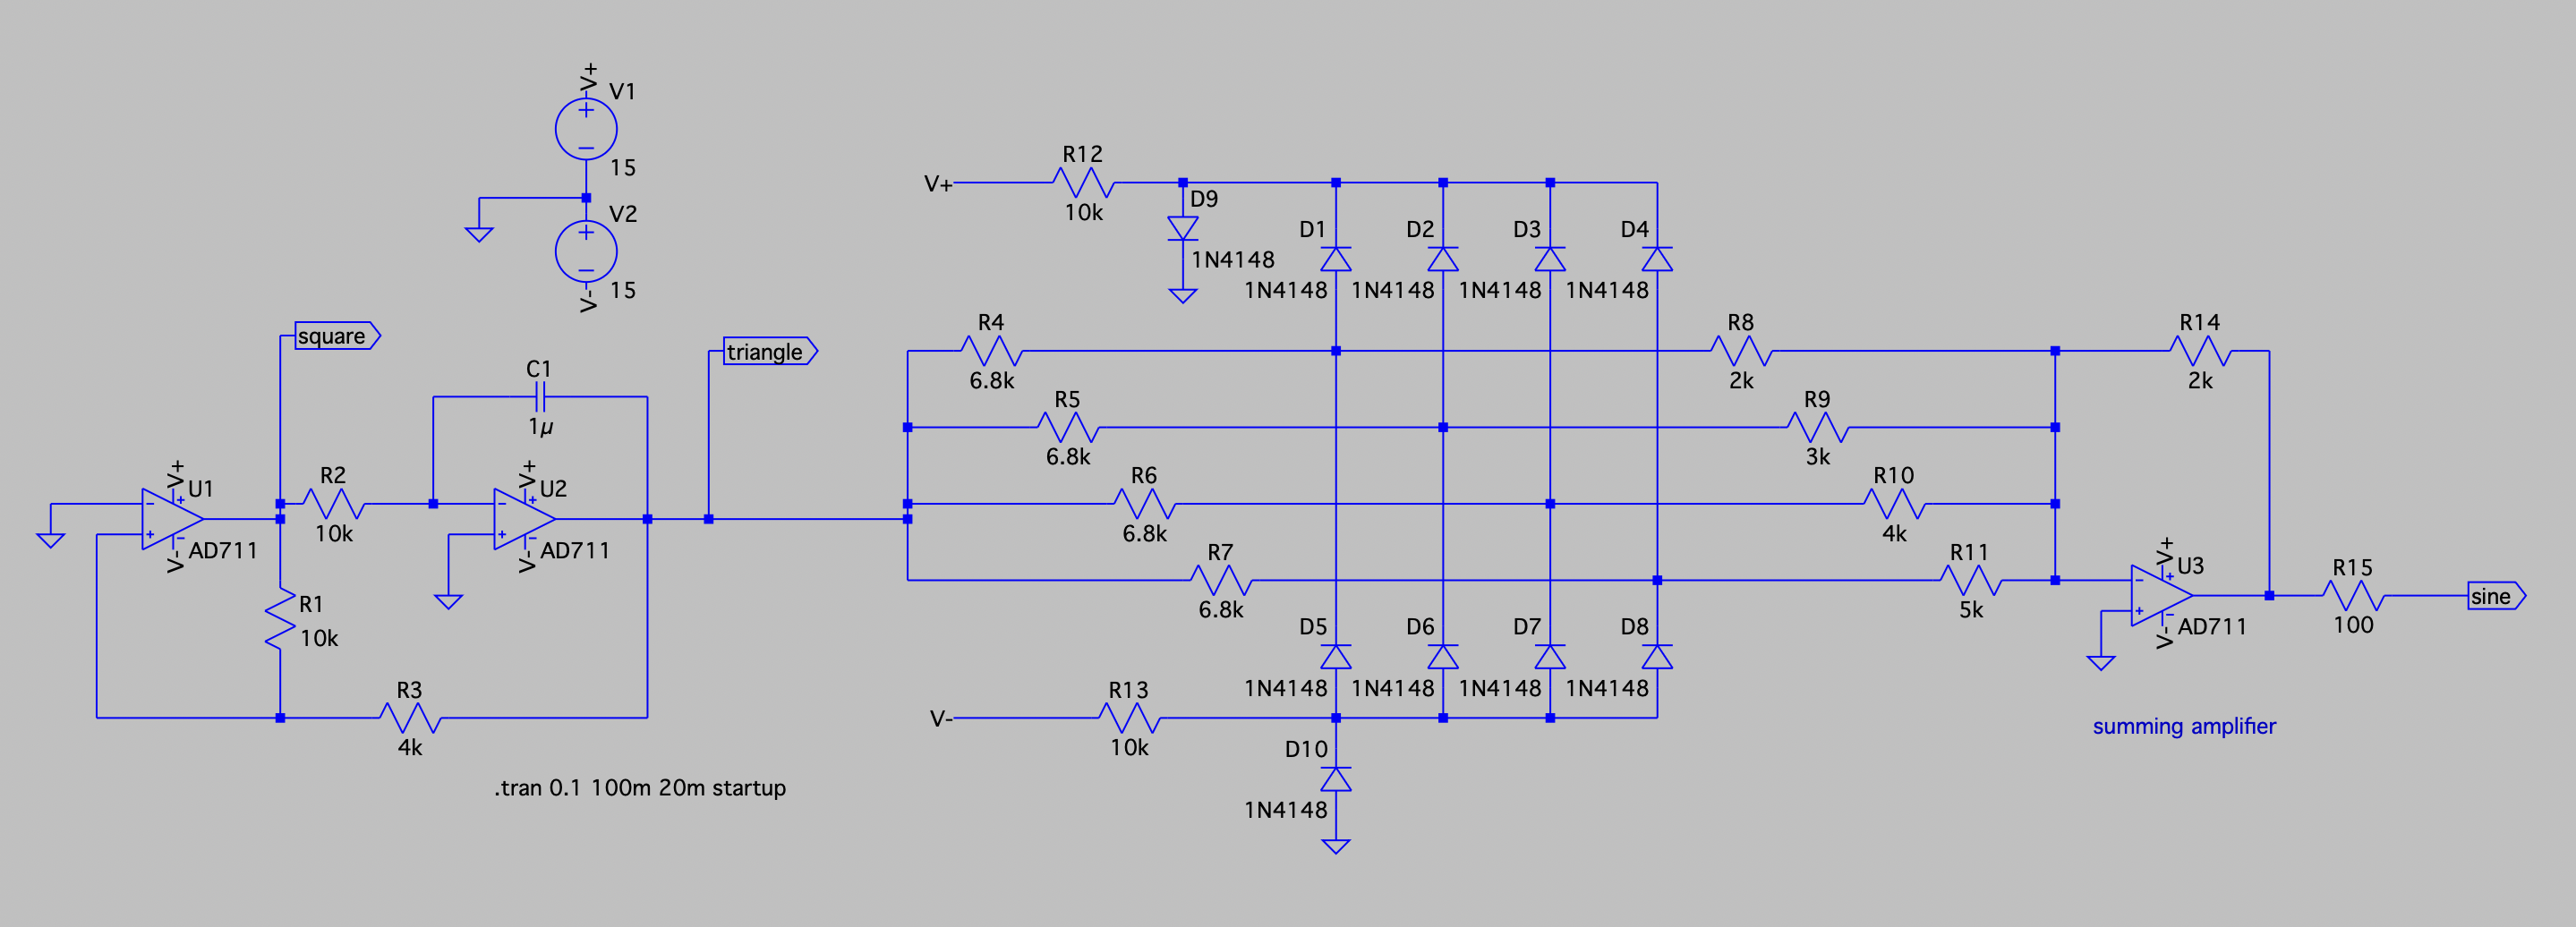
\includegraphics[width=1\textwidth]{schematic.png}
    \caption{Full schematic of the function generator circuit. U1 forms a square
    wave generator using a comparator with positive feedback. U2 is configured as
    an inverting integrator to generate a triangle wave. U3 shapes the triangle
    wave into a sine wave using a diode-resistor nonlinear network and summing
    amplifier configuration. Component values were selected to set the operating
    frequency to approximately $60$ Hz.}
    \label{fig:schematic}
\end{figure}

\noindent To analyze the quality of the generated sine wave, we performed
Fourier analysis to decompose the waveform into its frequency components.
The Discrete Fourier Transform (DFT) expresses a sampled signal $v(t_n)$
as a sum of weighted complex exponentials:
\begin{equation}
    V_k=\sum_{n-0}^{N-1}v(t_n)e^{-2\pi ikn/N},
\end{equation}
\noindent where $V_k$ is the complex amplitude of the $k$-th \cite{bounchaleun}. The
magnitude spectrum $|V_k|$ indicates the strength of each frequency component,
with the dominant peak corresponding to the fundamental frequency and
additional peaks representing harmonic distortion. Any deviation from a pure 
sine wave introduces higher-frequency harmonics into the signal \cite{williams}\cite{heinzen}. To quantify
this distortion, we compute the Total Harmonic Distortion (THD), which
which measures how much of the distortion is due to harmonics in the signal:
\begin{equation}
    \text{THD}=\frac{\sqrt{V_2^2+V_3^2+V_4^2+ \dots}}{V_1^2}.
    \label{eq:thd}
\end{equation}


% -------------------
% Methods and Results
% -------------------

\section{Methods and Results}

% Depending on the scientific article (and the style guide of the journal which publishes the
% research), these two sections may or may not be separate. Sometimes, the methods are
% described first and the results come second. Other times the results are shown first and
% the methods are described in a subsequent section. And finally, it sometimes makes sense
% to describe a method and then present the relevant results and then move onto the next
% method. You can choose which of these styles suits your lab report best as long as you
% include all the necessary information in a logical order.


\subsection{Methods}

% A description of what you did should be presented with enough detail to allow for your
% experiment to be repeated. Imagine that one of your classmates walks into lab and is
% handed your report. Would they be able to reproduce your results based on the details you
% provide in the methods section? You can use words, diagrams, pictures, etc (please use figure
% captions).


We built the circuit from Figure~\ref{fig:schematic} on a solderless breadboard powered using the
supply from a PB-505A set at $\pm18$ V. We used three AD711 op-amps, but any general purpose
op-amp should work. We observed the output waveforms using a Tektronix TBS10000C 2-Channel 
Oscilloscope and used the \texttt{Measure} function to record the amplitude, frequency, 
and rise/fall timesand duty cycle for the square wave. For the triangle wave, 
we visually checked for linearity and symmetry.\\

\noindent To evaluate the frequency content of the sine wave, we performed a Fast
Fourier Transform (FFT) on the waveform data using Python. We processed the data
using the \texttt{fft} function from the \texttt{scipy.fftpack} package to compute
the one-sided FFT magnitude spectrum. We identified the dominant frequency by 
locating the peak (excluding DC) and and the amplitudes at the 2nd-5th harmonics
to compute the Total Harmonic Distortion (THD) using Equation~\ref{eq:thd} \cite{heinzen}. 
We also performed a least-squares fit to the form:
\begin{equation}
    V(t)=A\sin(2\pi ft+\phi)+V_0
\end{equation}

\noindent using the \texttt{curve\_fit} function from the \texttt{scipy.optimize}
package, which allowed us to extract the amplitude $A$, frequency $f$ phase $\phi$,
and vertical offset $V_0$ of the signal. From these parameters, we computed the
RMS voltage of the waveform.\\

\noindent Before constructing the circuit, we ran transient simulations of each stage using LTSpice to verify
the expected waveform behavior (see Figure~\ref{fig:ltspice}).

\begin{figure}[H]
    \centering
    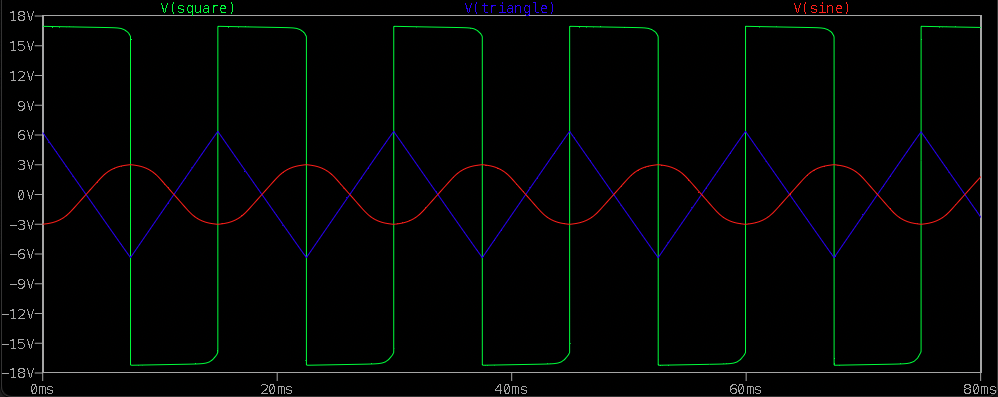
\includegraphics[width=.8\textwidth]{ltspice.png}
    \caption{Transient simulation showing the output waveforms at each stage
    of the function generator circuit.}
    \label{fig:ltspice}
\end{figure}


\subsection{Results}

% Please make sure to include all the measurements performed. When presenting results in
% a graph, please format the graph with legible axes that are titled and labeled with units
% as well as a figure caption that give all relevant information. This section should include
% measurements that prove that your project is working as expected.

To verify the performance of our function generator, we recorded the output waveforms
of all three stages, as shown in Figure~\ref{fig:waveforms}. Our results agree with our
LTSpice simulations. The square wave exhibited sharp transitions with measured rise
and fall times of approximately $25.75$ \si{\micro\second} and $24.60$ \si{\micro\second},
and near-symmetric duty cycles of $49.25$\% (positive) and $50.74$\% (negative), which
is expected from a properly biased comparator \cite{schertz}. The triangle showed linear charging and 
discharging behavior with consistent amplitude and frequency matching the square wave.\\

\begin{figure}[H]
    \centering
    \begin{subfigure}[b]{0.32\textwidth}
        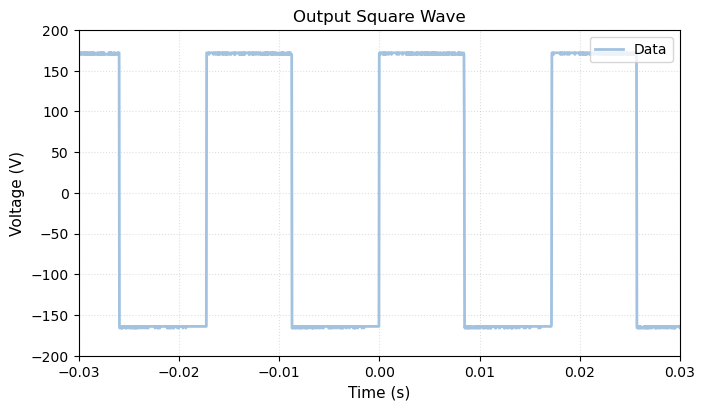
\includegraphics[width=\textwidth]{square_wave.png}
        \caption{Square wave}
        \label{fig:square_wave}
    \end{subfigure}
    \hfill
    \begin{subfigure}[b]{0.32\textwidth}
        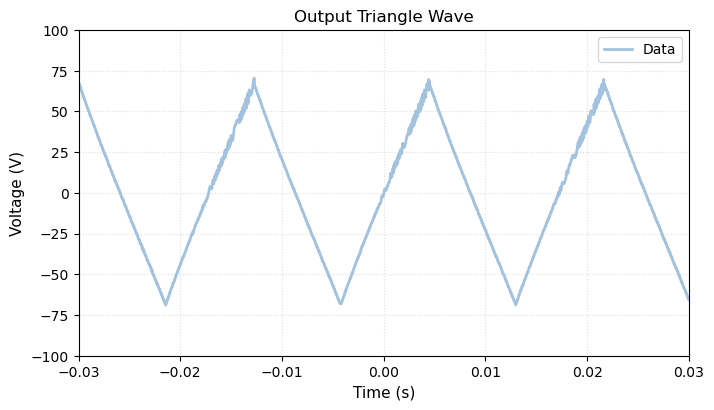
\includegraphics[width=\textwidth]{triangle_wave.png}
        \caption{Triangle wave}
        \label{fig:triangle_wave}
    \end{subfigure}
    \hfill
    \begin{subfigure}[b]{0.32\textwidth}
        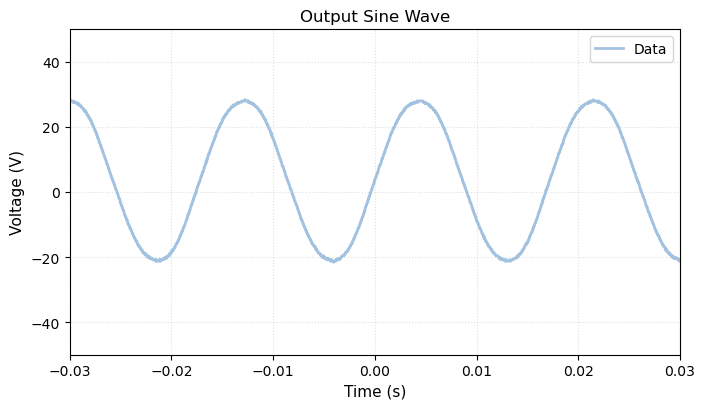
\includegraphics[width=\textwidth]{sine_wave.png}
        \caption{Sine wave}
        \label{fig:sine_wave}
    \end{subfigure}
    \caption{Oscilloscope waveforms from each stage of the function generator circuit ($f=58.08$ Hz).}
    \label{fig:waveforms}
\end{figure}


\noindent We identified the fundamental frequency from the FFT spetrum as $62.5$
Hz, with secondary peaks at $125.0$ Hz, $187.5$ Hz, $250.0$ Hz, and $312.5$ Hz 
corresponding to the 2nd-5th harmonics. We computed the Total Harmonic Distortion
to be $11.44$\%, which suggests our passive diode network had reasonable sine
shaping performance \cite{williams}. The FFT magnitude spectrum is shown in Figure~\ref{fig:fft_mag}.

\begin{figure}[H]
    \centering
    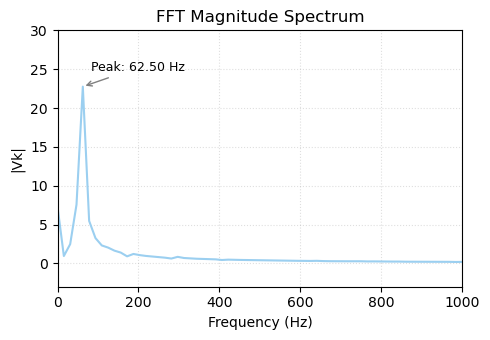
\includegraphics[width=.7\textwidth]{fft_mag.png}
    \caption{FFT magnitude spectrum showing the fundamental at 62.5 Hz and harmonic distortion.}
    \label{fig:fft_mag}
\end{figure}

\noindent We used a nonlinear least-squares fit to the sine output to get the
following parameters: $A=25.02$ V, $=58.16$ Hz, $\phi=-0.014$ rad, and $V_0=4.62$ V.
The computed RMS voltage of $17.69$ V was close to the measured $17.25$ V, confirms the
waveform's sinusoidal nature. Figure~\ref{fig:sine_fit} shows the original waveform
and fit.

\begin{figure}[H]
    \centering
    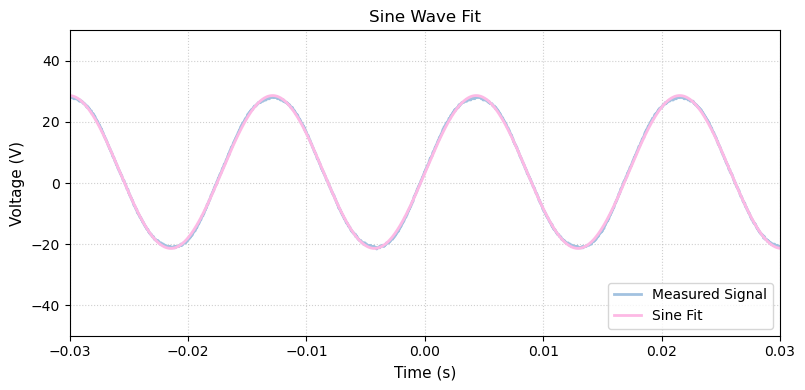
\includegraphics[width=.75\textwidth]{sine_fit.png}
    \caption{Nonlinear least-squares fit to the sine wave output.}
    \label{fig:sine_fit}
\end{figure}

\noindent The recorded frequency from the oscilloscope was approximately
$58.08$ Hz, is close to the fitted value of $58.16$ Hz and is within
reasonable error of FFT-detected $62.5$ Hz fundamental. These small differences
are likely due to resolution in the FFT bins and oscilloscope sampling rate. 
We also observed minor deviations during longer runtimes, which
could affect waveform symmetry and stability. Despite these factors, the 
generator produced consistent outputs across all stages, and our results
aligned closely with theoretical expectations.

% ----------
% Conclusion
% ----------

\section{Conclusion}

% Quickly summarize your results and their relevance to electronic methods or techniques. The
% reader should walk away with a clear “take-home message” after reading your conclusion. If
% something went wrong with your experiment and you didn’t get conclusive results, or your
% results disagree with theory, this is your chance to explain what went wrong and propose an
% improvement to the experiment.

In this project, we successfully designed and built a function generator
circuit capable of producing square, triangle, and sine waveforms using
op-amp stages and passive shaping components. The comparator-inverter
loop reliably generated a square wave, which was integrated into a traiangle
waveform and subsequently converted into a sine wave using a diode resistor
network and summing amplifier. Our measurements showed consistent waveform
frequency across all stages. The output sine wave had a measured frequency
of approximately $58.08$ Hz, with the nonlinear curve yielding $58.16$ Hz and 
FFT-based analysis detecting a $62.5$ Hz peak. The total harmonic distortion
was $11.44$\%, which indicates moderate deviation from a pure sine likely due
to diode nonidealities, waveform asymmetries, and component tolerances.\\

\noindent Small discrepancies between computed and measured frequencies may
have resulted from oscilloscope sampling limitations, FFT bin resolution, and
phase noise in the signal. Additionally, the slight mismatch in our power
supply rails (e.g., $\pm 17.98$ V vs. $\pm18.00$ V) resulted in asymmetry that likely
affected integration slopes and sine shaping. Additionally, component
tolerances (especially resistors in the feedback paths) and thermal drift
over time also contributed to deviation from ideal behavior \cite{seddik}.\\

\noindent Future improvements could include using tigher-tolerance components, 
adding trimmer potentiometers for threshold calibration, and incorporating
active filter stages to better suppress harmonics \cite{fallows}. Refinement of waveform
quality can also be tested by adjusting component values such as $R_2$ to
modify the integrator slope and output frequecy, or by fine-tuning the supply
voltage $V_\pm$ to control the amplitude. Finally, we suggest improving
power supply regulation and thermal compensation to improve stability and
reduce long-term drift.\\


\section*{Acknowledgements}

We would like to thank our laboratory instructor, Dr. Heinzen, and our teaching 
assistant, Kyle Gable, for their guidance and support through these labs. Their 
assistance and feedback were invaluable in helping us understand the experimental 
procedures and circuit concepts. We also appreciate the department's laboratory 
facilities and equipment, which made these experiments possible.

\bibliographystyle{plain}  % or another style like ieee, unsrt, etc.
\bibliography{refs}        % refs.bib (no .bib in the command)

\end{document}
